% Experiments

\label{sec:experiments}

The midway experiments evaluate the completed PPO, SAC, and TD3 baseline matrix. The purpose is not to evaluate the final GRPO-control method, which is left for the final project stage, but to validate the experimental pipeline and establish a reproducible baseline foundation for the later GRPO comparison.

\subsection{Baseline Matrix and Result Validation}
\label{sec:experiments-validation}

The experiment matrix consists of three algorithms, three environments, and five random seeds. The algorithms are PPO, SAC, and TD3. The environments are \texttt{cartpole\_swingup}, \texttt{acrobot\_swingup}, and \texttt{car\_racing\_continuous}. The seeds are $0,1,2,3,4$, giving
\[
3 \text{ algorithms} \times 3 \text{ environments} \times 5 \text{ seeds}
=
45 \text{ runs}.
\]

The final report-facing notebook validates that all 45 expected algorithm--environment--seed combinations are present. It also confirms that the result set contains 900 evaluation rows, that all three algorithms and all three environments are represented, and that all evaluation rows have status \texttt{completed}. The reported figures and summaries are therefore based on a complete midway baseline matrix rather than a partial subset of experiments.

\subsection{Baseline Learning Curves}
\label{sec:experiments-learning-curves}

Figure~\ref{fig:midway-vector-baselines} shows the midway learning curves for the two vector-control environments. The horizontal axis gives the number of training steps before evaluation, and the vertical axis gives the undiscounted evaluation episode return. The vector-control experiments use a midway budget of 20,000 training steps. The CarRacing experiments use a shorter budget of 10,000 training steps and are included in the same validated result pipeline.

\begin{figure}[t]
  \centering
  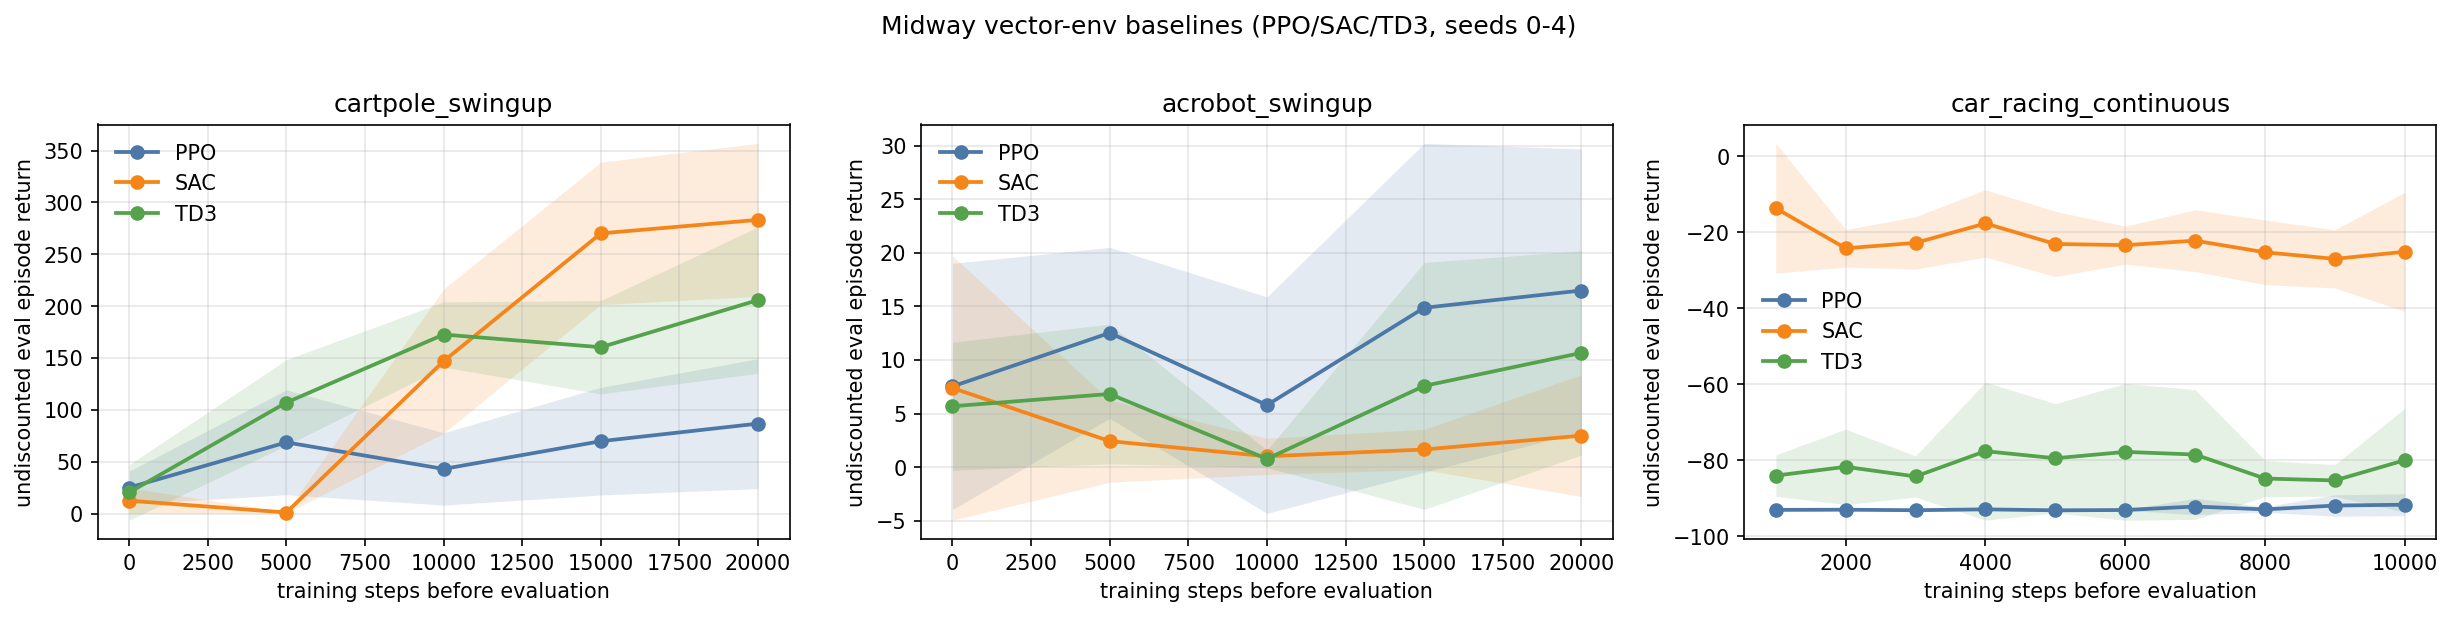
\includegraphics[width=\linewidth]{../figures/midway/midway_vector_env_baselines.png}
  \caption{Midway PPO, SAC, and TD3 baseline learning curves for the vector-control environments.}
  \label{fig:midway-vector-baselines}
\end{figure}

The clearest learning signal appears in \texttt{cartpole\_swingup}. At the midway budget, SAC obtains the highest mean final return, followed by TD3. Both methods improve from the first to the final evaluation point, while PPO ranks lower in the final evaluation summary.

The results for \texttt{acrobot\_swingup} are more modest. PPO obtains the highest mean final return at the midway budget, followed by TD3 and SAC. PPO and TD3 show positive development across the run, while SAC does not show the same improvement under the present short setup. This suggests that the environment is more difficult under the selected midway budget and may require longer training or tuning before stronger conclusions can be drawn.

For \texttt{car\_racing\_continuous}, the final returns remain negative for all three algorithms, which is expected under a short CNN-based midway budget. SAC obtains the best mean final return among the CarRacing baselines, followed by TD3 and PPO. The main midway result for CarRacing is therefore not high performance, but that the project-side CNN pipeline runs successfully for PPO, SAC, and TD3 and that the image-based environment is included in the same validated baseline matrix as the vector-control environments.

\subsection{Interim Interpretation and Limitations}
\label{sec:experiments-interpretation}

Overall, the experiments show that the baseline pipeline is functional and complete. The project can run PPO, SAC, and TD3 on all three environments, collect results for five seeds, validate the expected result matrix, and generate learning curves from the stored evaluation data. This establishes the comparison basis required for the final GRPO-control evaluation.

The results should be interpreted cautiously. The training budgets are short, and no hyperparameter optimization was performed. Differences between PPO, SAC, and TD3 may therefore reflect both algorithmic differences and the selected baseline configurations. The results also show variation across seeds and evaluation points, which is expected in reinforcement learning due to initialization, exploration, and environment interaction.

The midway experiments do not answer the full research question of the project. They do not evaluate the final GRPO-control method and should not be used to claim general algorithmic superiority. Their role is to establish a reproducible baseline foundation. In the final stage, the GRPO-control method should be evaluated on the same environments, with the same seed structure and evaluation metric, so that the comparison with PPO, SAC, and TD3 remains consistent.
